\chapter{Introduction\label{cha:chapter1}}

The Internet has become an essential part of our daily lives in different sectors business, social communication, healthcare, etc. It has revolutionized our economy and society and therefore considered to be at the top of the technological revolution in the current century. The success of the Internet can be seen by its traffic growth. The monthly global Internet traffic is expected to quadruple between 2010 and 2015 increasing from about 20.2 exabytes to 80.5 exabytes (one exabyte equals one billion gigabytes)\cite{cisco1}. Indeed, this growth indicates how huge the content (and rapidly increasing) that is uploaded and consumed is. Around one million minutes of video content will cross the network per second in 2015 \cite{cisco1}. About one hour of YouTube videos are being uploaded per second and more than four billion views per day\cite{youtube1}. The video-sharing content in YouTube is only one example of a huge number of distributed contents on the Internet provided by various content delivery platforms. These platforms provide different types of contents, i.e. contents are heterogeneous and can be anything, e.g. video, multimedia, books, etc. 

The recent growth of multimedia content offered by multiple professional content providers (e.g. \ac{IPTV} or mobile TV provider), available in several multimedia-based social networking communities or distributed in various user devices, seems to be clear evidence for the need of an efficient multimedia provisioning framework that supports efficient and personalized provisioning and discovery mechanisms of multimedia content information compared to the classical client-server provisioning systems. This thesis will address the increase of the wealth of distributed multimedia content either in a controllable network or in a user private network. The challenge is to provide users with technical means for rapid and instant access to relevant, trustworthy multimedia content information and enriched personalization.

Nowadays, devices such as PCs, smartphones, positioning devices, health monitors in our environment, are expected to work with high levels of independence, performing programmed actions that benefit their users in everyday life. In order to meet this set of requirements, these different devices are connected together to perform certain tasks. This concept is known as \ac{M2M} communication. \ac{M2M} is a concept that defines the rules and relations between devices while cooperating with each other. It implies a highly automated usage of a set of devices simultaneously, without much need for human interaction. With the increase of computational power, it is even possible to run different \ac{M2M} tasks on various consumer electronics (e.g. television sets, set-top boxes), however smartphones are still more frequently used in \ac{M2M} domain.

The aim of this thesis is to develop a context-aware framework, in which the context information of multimedia content environment (such as location and time) is considered and embedded into the captured multimedia content as content information or metadata. The proposed framework uses \ac{M2M} concept, which provides several resources such as sensor information like temperature, \ac{GPS} data, and so on. These resources can be used to enrich the metadata of the captured content. The motivation behind this work is due to the lack of context/content-aware storage management in the current Internet architecture which is one of its fundamental limitations \cite{ec1}. The consumer, who is interested in a particular multimedia content service, submits the request with defined conditions (e.g. time, location, content provider, etc.) that are evaluated against multimedia context information in order to deliver the associated multimedia content information (e.g. content resources, description, etc.). User-specific conditions can be published once or updated regularly. The multimedia content service shall examine user-specific conditions and notifies the user with the matched multimedia content. Therefore, an efficient interaction model between consumer and the service will be developed. Furthermore, an end-to-end multimedia content service will be implemented in order to demonstrate the developed concept.

\section{Motivation\label{sec:moti}}

Context-aware systems can help people in many areas of daily life in order to plan their daily schedule, to make the right decisions  and to perform other tasks for them.

Due to the fact of increased computing power of today's mobile devices, tasks are now performed that were not possible a few years ago. For these devices, with their increasingly complex applications, context-aware behaviour is very important. Reliable, easy context-aware systems are required because of the explosive growth of content consumption from mobile devices and social networks and the consumer expectation of content availability on various devices. According to a statistic result reported by The Nielsen Company, U.S mobile video viewers have grown from 23 million in the third quarter of 2010 to 31 million in the third quarter of 2011 \cite{mobile-media-report}.

\ac{M2M} technology is growing fast and  will be available everywhere in the near future. Such technology will help to enrich context information associated with multimedia content.

There are several reasons for working on this diploma thesis. On one hand, there is no correlation nowadays between content and context supported by the current Internet architecture. However, there is a demand for solutions or products that simplify the usage of the distributed content based on a specific type of context. The unavailability of such solutions or products is one of the main motivations behind this thesis. Within the context of this thesis, a new valid prototyping for context-aware content management framework will be developed. Therefore this thesis will set the ground for future investigations and will also be used as a cornerstone and give directions for better designed and acceptable solutions.

On the other hand, working on this thesis gives me the chance to get in-depth knowledge and hands-on experience of a hot topic that will evolve, improve and develop in the years to come and eventually become an integral part of normal lifestyle.

\section{Objective\label{sec:objective}}

The main objective of this thesis is to develop a contextual content management framework in which the context information/metadata is created automatically during content capturing and relies on local, distributed sensing information. The framework will support the correlation and synchronization of context information and multimedia content stream. In order to deliver the content to various devices, the distribution mechanism will be implemented. The distribution mechanism should be aware of the device properties i.e screen resolution or internet speed. For context enrichment, the framework should provide a mechanism that uses the benefits of \ac{M2M} concept.

Figure \ref{fig:oarch} shows the main component of the platform:
\begin{figure}[htb]
  \centering
  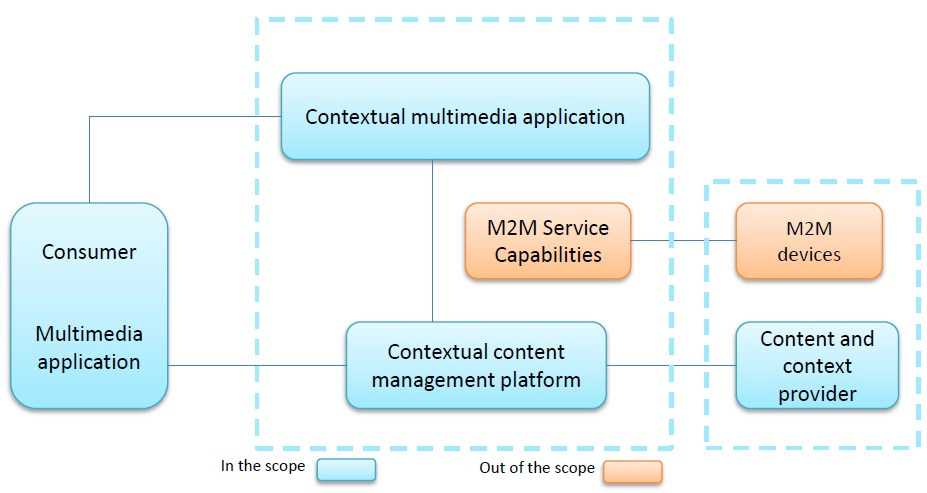
\includegraphics[scale=0.5]{DA-OverallArchitecture.jpg}\\
  \caption{Overall Architecture}
  \label{fig:oarch}
\end{figure}


\section{Scope\label{sec:scope}}

Due to the lack of time and possible wide range of technologies which have been mentioned above, the objective will be defined here in detail to decide what should be developed in this thesis.

The scope of this thesis is to manage the relationship between content and context. In order to manage this relationship, this thesis will study the state of the art of data model description and then choose the appropriate one. The thesis should integrate the \ac{M2M} concept for context enrichment.


The activities in this thesis are outlined as follows:
	\begin{itemize}
		\item Act. 1: Study of the state of the art of data model format, context description language
				\vspace{-0.1in} 
		\item Act. 2: Defining a concept for discovering sensors (locally deployed or with \ac{M2M} platform), subscriptions and notification for sensor information.
				\vspace{-0.1in} 
		\item Act. 3: Investigate the process of automatic creation of context information and data fusion (correlation between context and content)
				\vspace{-0.1in} 		
		\item Act. 4: Design the required management and delivery platforms 
    			\vspace{-0.1in} 
		\item Act. 5: Examine the available open sources for content management systems and \ac{HTTP} based streaming servers
 				\vspace{-0.1in} 
		\item Act. 6: Based on available open source solutions, develop an end-to-end platform that enables content provider(mobile app.) to capture multimedia content with the associated context information and publish this content to the server and allow consumers(mobile app. or web based) to discover and subscribe to multimedia content according to defined conditions. 
    			\vspace{-0.1in} 
    	\item Act. 7: Develop an end-to-end application to evaluate the implemented functionality
%		\item Act. 8: Validate the implementation through an end-to-end deployment scenario that is planned to be deployed in the FOKUS open \ac{EPC} or \ac{MTC} playground. In the first deployment scenario, the quality of content streaming to the consumer or network selection will be instantly identified according to user and network policies. In the second deployment scenario, content-related context information – in particular geographical and time information of multimedia content stream – can be considered as collaborative crowd sourcing with multimedia content that can enrich any \ac{MTC} platform.
    \end{itemize}

\pagebreak

Figure \ref{fig:inout} shows inputs and outputs for this thesis:

\begin{figure}[htb]
  \centering
  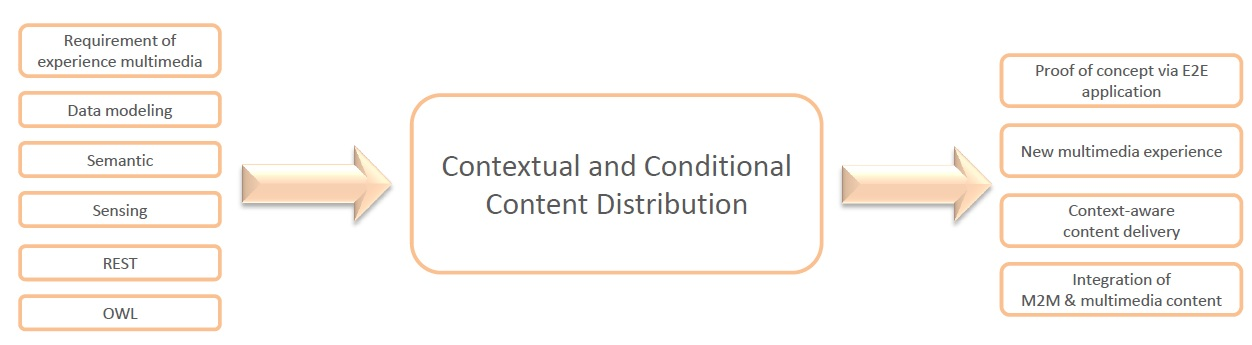
\includegraphics[scale=0.4]{Inp_Out.jpg}\\
  \caption{Inputs \& Outputs}
  \label{fig:inout}
\end{figure}

By studying these tasks, the goal is to draw conclusions about the best practices in this domain, and design the framework that will establish the basis for its further development and future implementation.

%\section{Impact\label{sec:intro_impact}}

%\section{Methodologie\label{sec:intro_meth}}
\section{Outline\label{sec:intro_out}}
In chapter \ref{cha:chapter2}, the background and relevant technologies for this thesis will be presented. Chapter \ref{cha:chapter3} deals mainly with the functional and non functional requirements for the framework to be developed. Chapter \ref{cha:chapter4} represents the most comprehensive and important part of this thesis. This chapter provides a prototype design for the framework based on the requirements identified in chapter \ref{cha:chapter3}. Chapter \ref{cha:chapter5} deals with the prototype implementation of the design presented in chapter \ref{cha:chapter4}. Next, the evaluation and conclusion follows in chapter \ref{cha:chapter6} and chapter \ref{cha:chapter7} respectively.
%\section{Use case\label{sec:use_case}}
%
%For better understanding the functionality of the proposed platform, an example is discussed in this section as a use case scenario.
%
%A user as a content provider captures a live event (e.g. demonstration, car race, marathon, Tour de France, etc.) using an application on a GPS capable smartphone. While capturing, the application also collects context information (e.g. location, acceleration, temperature, time, etc.). Later the user uploads the captured content with its context information to the platform.
%
%Let's consider the Tour de France as an example for the uploaded content in the following. Any content consumer, who is interested in a specific uploaded content that has been captured in a specific place on the road of the Tour (e.g. Les Essarts town which is located in western France), searches for the content by specifying some related information such as time range, location and `Tour de France` as search string. The platform will then give the user a list of all content that match the specified criteria. The user can select any of the provided contents.
%
%\section{Requirement\label{sec:use_case}}
%The above use case is a textual representation illustrating a sequence of events, which imply different requirements. Figure \ref{fig:req} shows the requirement.
%\begin{figure}[htb]
%  \centering
%  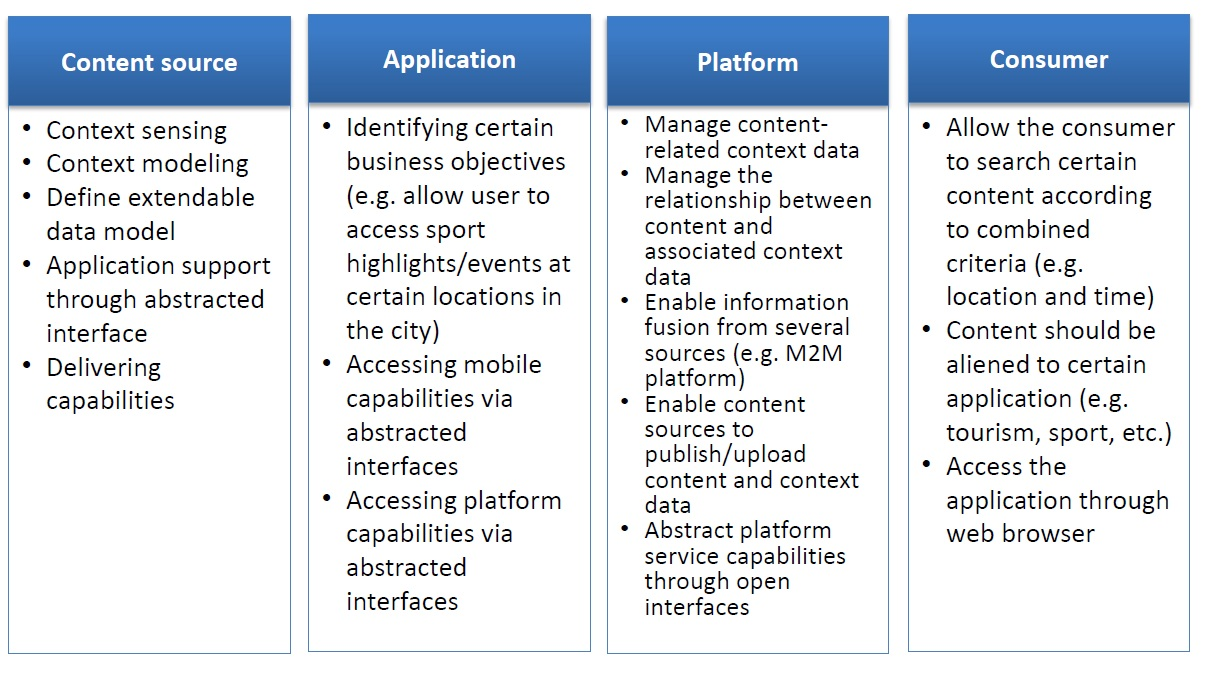
\includegraphics[scale=0.4]{Requirements.jpg}\\
%  \caption{Requirements}
%  \label{fig:req}
%\end{figure}

%\section{Plan\label{sec:plan}}
%
%The processing time of a thesis from the application until the completion is six months. A rough schedule with milestones is shown in Figure \ref{fig:plan}. The chart provides a big picture for the conduct of the dissertation, which will be refined over time.
%During the processing time there are regular meetings between the candidate and supervisors.
%\begin{figure}[htb]
%  \centering
%  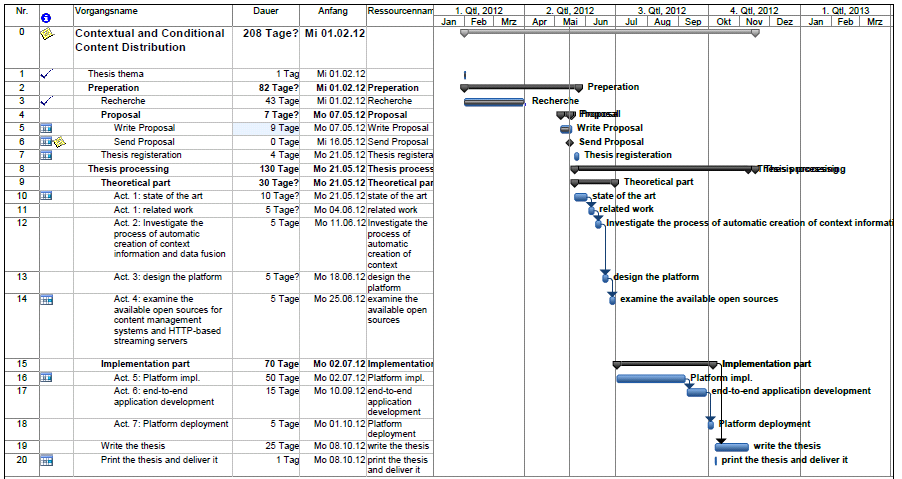
\includegraphics[scale=0.6]{Plan_new1.PNG}\\
%  \caption{Plan}
%  \label{fig:plan}
%\end{figure}
